\documentclass{report}
\usepackage[margin=0in,paperwidth=10.5in,paperheight=6.125in]{geometry}
\usepackage{tikz}
\usetikzlibrary{calc}
\usetikzlibrary{decorations.pathreplacing}
\pagestyle{empty}
\hoffset 0.125in
% \voffset -0.375in
\begin{document}
% Helper commands for these slides
    \newcommand \sboxOne{
    	\mbox{
    		$
    		\begin{array}{|c|c|c|c|c|}\hline
    				& 00 & 01 & 10 & 11 \\ \hline
    			00 & 01 & 11 & 10 & 11 \\		\hline
    			01 & 11 & 10 & 01 & 00 \\		\hline
    			10 & 00 & 10 & 01 & 11 \\		\hline
    			11 & 11 & 01 & 11 & 10 \\		\hline
    		\end{array}
    		$
    	}
    }
    
    \newcommand \sboxTwo{
    	\mbox{
    		$
    		\begin{array}{|c|c|c|c|c|}\hline
    				& 00 & 01 & 10 & 11 \\ \hline
    			00 & 00 & 01 & 10 & 11 \\		\hline
    			01 & 10 & 00 & 01 & 11 \\		\hline
    			10 & 11 & 00 & 01 & 00 \\		\hline
    			11 & 10 & 01 & 10 & 11 \\		\hline
    		\end{array}
    		$
    	}
    }
    
 

    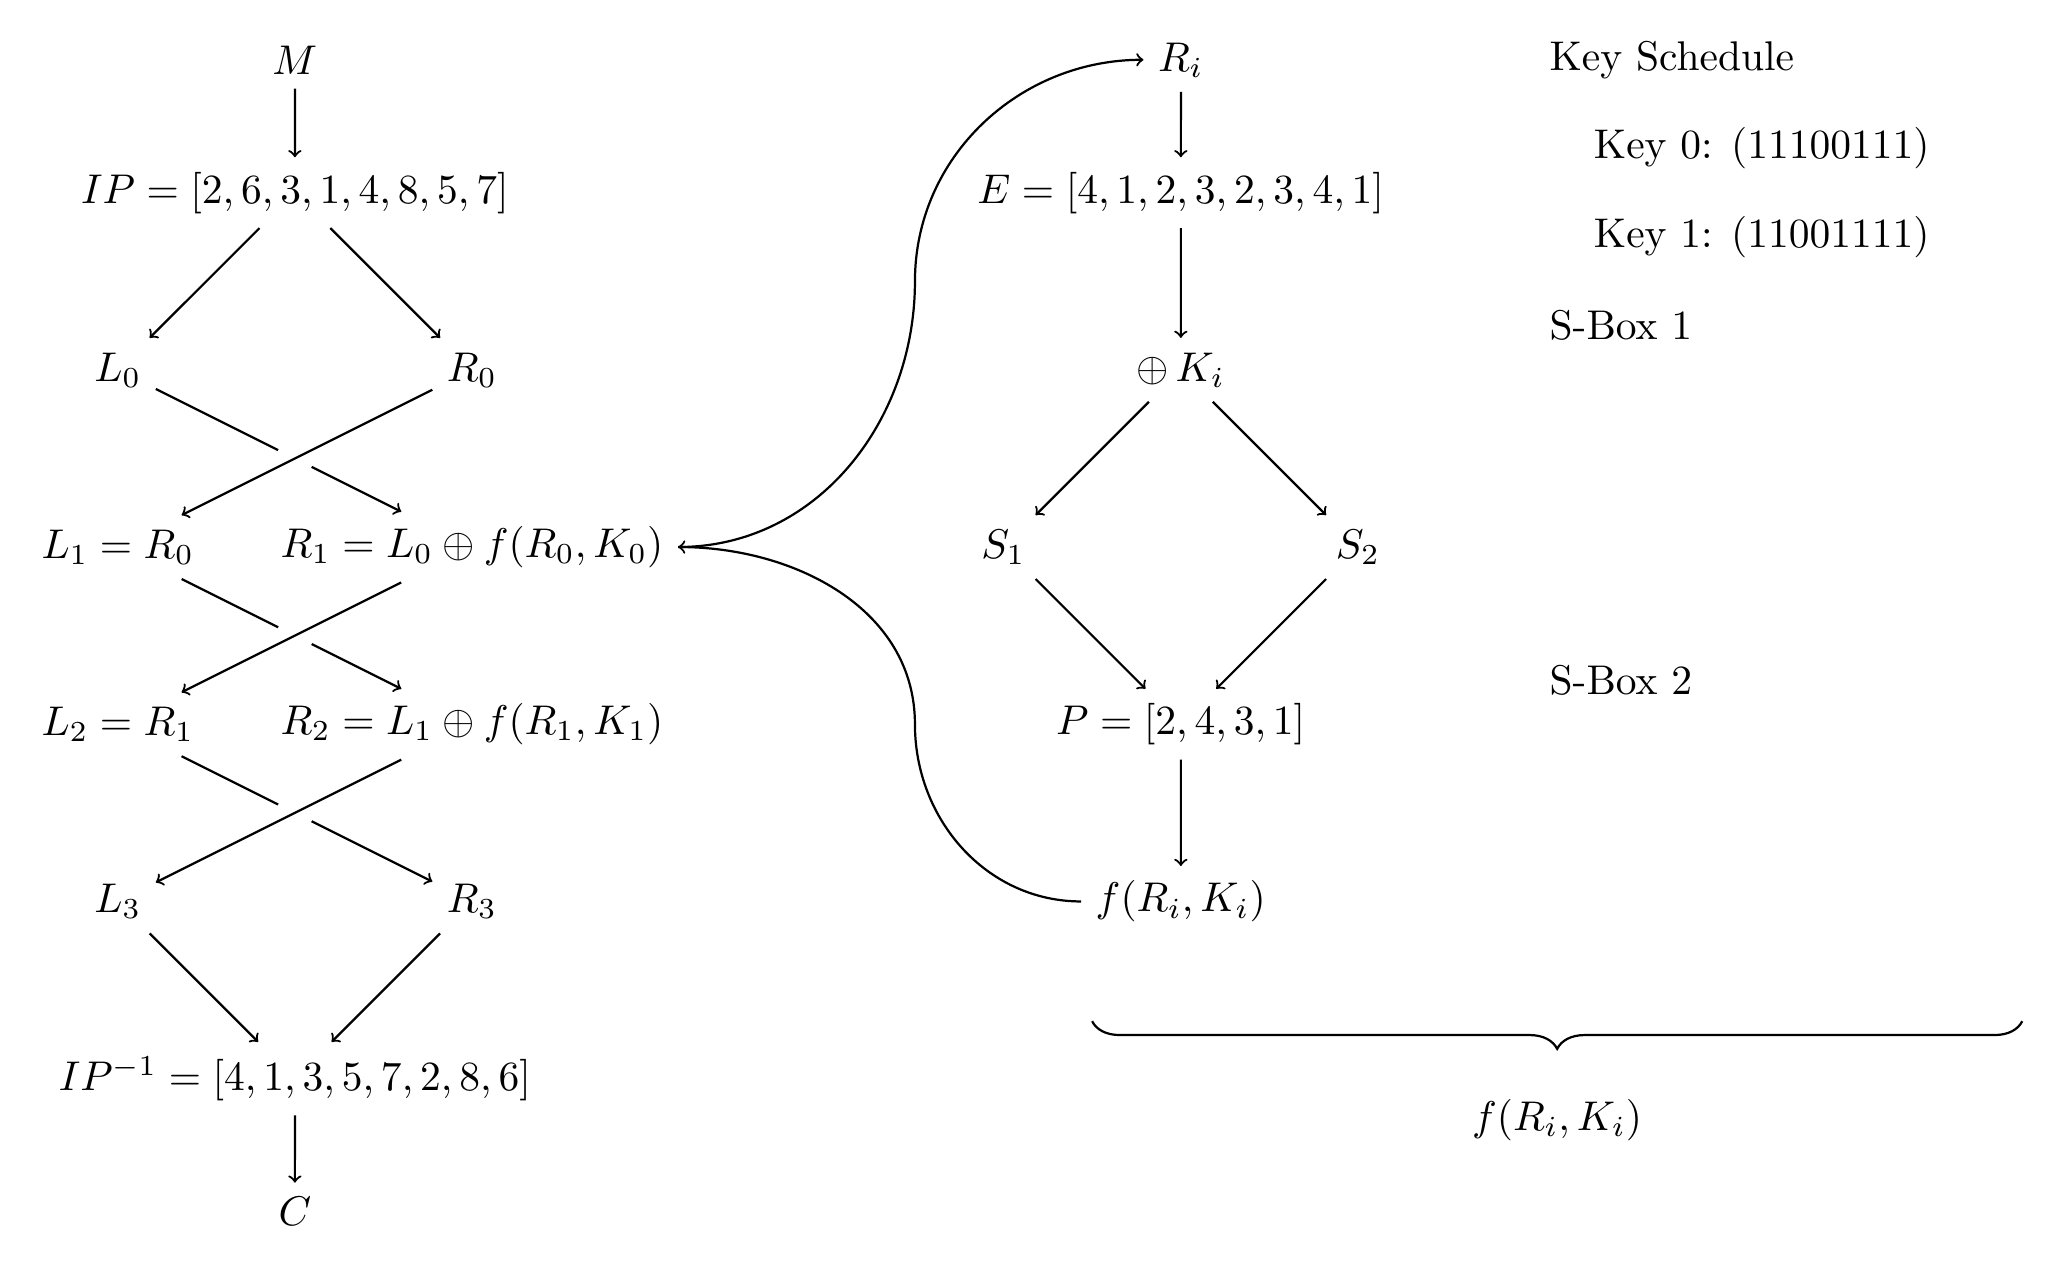
\begin{tikzpicture}[
        scale=2.25,
        every node/.style={scale=1.5}
    ]
    % Helper Grid    
        % \draw[thick,red,dashed,opacity=0.5] (0,0) grid (0.8\textwidth,0.7\textheight);
        % \foreach\x in {0,...,6}{
        %     \node[anchor=north] at (\x,0) {\x};
        %     \node[anchor=east] at (0,\x) {\x};
        % }

    % Key Schedule
        \node[anchor=west] at (8,5.75) {Key Schedule};
        \node[anchor=west] at (8.25,5.25) {Key 0: (11100111)};
        \node[anchor=west] at (8.25,4.75) {Key 1: (11001111)};

    % S-Boxes
        \node[anchor=west] at (8,4.25) {S-Box 1};
        \node[anchor=north west] at (8.25,4) {\sboxOne};
        \node[anchor=west] at (8,2.25) {S-Box 2};
        \node[anchor=north west] at (8.25,2) {\sboxTwo}; 
     
    % Main Rounds Diagram
        % Message and Initial Permutation
            \node (M) at (1,5.75) {$M$};
            \node (IP) at (1,5) {$IP=[2,6,3,1,4,8,5,7]$};
        % Feistel nodes
            \node (L0) at (0,4) {$L_0$};
            \node (R0) at (2,4) {$R_0$};
            \node (L1) at (0,3) {$L_1=R_0$};
            \node (R1) at (2,3) {$R_1=L_0\oplus f(R_0,K_0)$};
            \node (L2) at (0,2) {$L_2=R_1$};
            \node (R2) at (2,2) {$R_2=L_1\oplus f(R_1,K_1)$};
            \node (L3) at (0,1) {$L_3$};
            \node (R3) at (2,1) {$R_3$};
        % Inverse Permutation and Cipher Text
            \node (IPI) at (1,0) {$IP^{-1}=[4,1,3,5,7,2,8,6]$};
            \node (C) at (1,-0.75) {$C$};
        % Connectors
            \draw[thick,->] (M) -- (IP);
            \draw[thick,->] (IP) -- (L0);
            \draw[thick,->] (IP) -- (R0);
            \draw[thick,->] (L0) -- (R1);
            \fill[white] ($(L0)!0.5!(R1)$) circle (3pt);
            \draw[thick,->] (R0) -- (L1);
            \draw[thick,->] (L1) -- (R2);
            \fill[white] ($(L1)!0.5!(R2)$) circle (3pt);
            \draw[thick,->] (R1) -- (L2);
            \draw[thick,->] (L2) -- (R3);
            \fill[white] ($(L2)!0.5!(R3)$) circle (3pt);
            \draw[thick,->] (R2) -- (L3);
            \draw[thick,->] (L3) -- (IPI);
            \draw[thick,->] (R3) -- (IPI);
            \draw[thick,->] (IPI) -- (C);
    % One round of the round function
        % Function Header
            \draw[thick,decorate,decoration={brace,mirror,amplitude=10pt},yshift=-5pt] (5.5,0.5) -- (10.75,0.5)node[pos=0.5,below,yshift=-15pt]{$f(R_i,K_i)$};
        % Nodes
            \node (F) at (6,5.75) {$R_i$};
            \node (E) at (6,5) {$E = [4, 1, 2, 3, 2, 3, 4, 1]$};
            \node (K) at (6,4) {$\oplus\, K_i$};
            \node (S1) at (5,3) {$S_1$};
            \node (S2) at (7,3) {$S_2$};
            \node (P) at (6,2) {$P=[2,4,3,1]$};
            \node (FRK) at (6,1) {$f(R_i,K_i)$};
        % Connectors
            \draw[thick,->] (R1) to[out=0,in=270] (4.5,4.5) to[out=90,in=180] (F);
            \draw[thick,->] (F) -- (E);
            \draw[thick,->] (E) -- (K);
            \draw[thick,->] (K) -- (S1);
            \draw[thick,->] (K) -- (S2);
            \draw[thick,->] (S1) -- (P);
            \draw[thick,->] (S2) -- (P);
            \draw[thick,->] (P) -- (FRK);
            \draw[thick,->] (FRK) to[out=180,in=270] (4.5,2) to[out=90,in=0] (R1);
    \end{tikzpicture}
\end{document}